\subsection{Background Distributions in {\tt GENE}}
    The source code for {\tt GENE} can be found in {\tt src/}. This implementation builds on the GPU support branch of the development version of {\tt GENE}, as it comes the closest to having fully functional support for varied background distributions.
    
    This branch of {\tt GENE} features options for background distributions (e.g. Maxwellian/shifted Maxwellian/etc.) through classes {\tt dist\_eq\_*\_t} (in a corresponding {\tt dist\_eq\_*\_m} module) that extend the base distribution class {\tt dist\_eq\_t} (part of the {\tt dist\_eq\_base\_m} module). (See Figure \ref{class structure before damping}) For each new species that uses such a background distribution, a new instance of this class is created.

    \begin{figure}[!h]
    \centering
    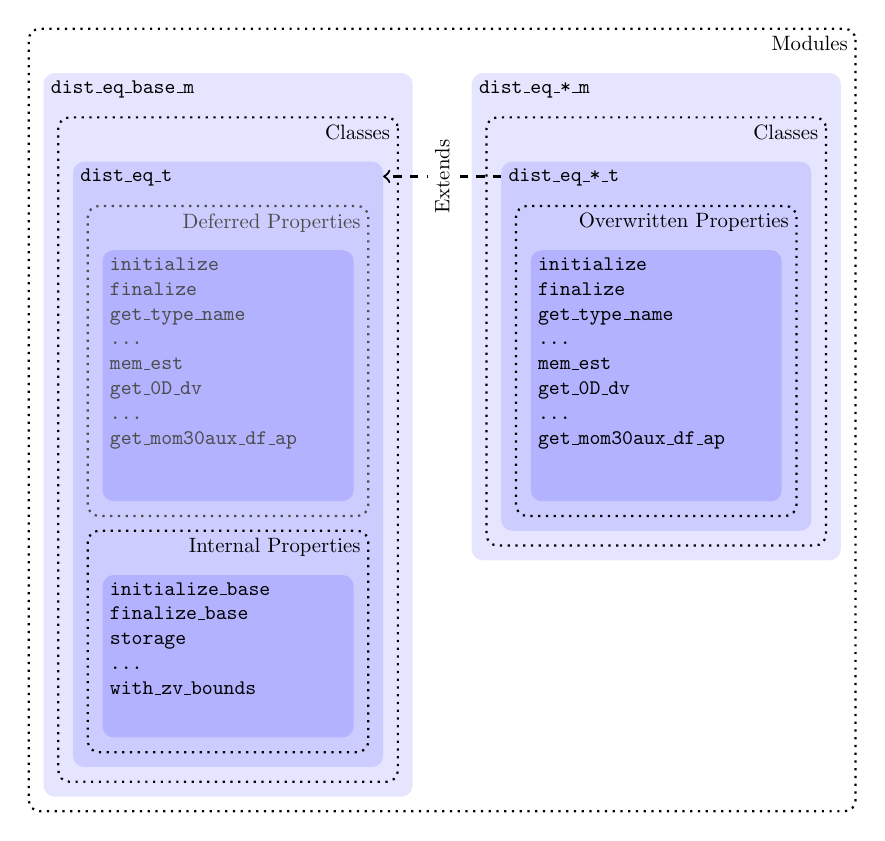
\begin{tikzpicture}[scale = 0.75, every node/.style = {scale = 0.75}, every text node part/.style = {align = left}]
        \draw[rounded corners, dotted, thick]
            (13.75, 0.75) node[below left] {Modules}
            rectangle
            (-0.25, -12.5);
            \fill[rounded corners, fill = blue!10]
                (0, 0) node[below right] {\tt dist\_eq\_base\_m}
                rectangle
                (6.25, -12.25);
                \draw[rounded corners, dotted, thick]
                    (6, -0.75) node[below left] {Classes}
                    rectangle
                    (0.25, -12);
                    \fill[rounded corners, fill = blue!20]
                        (0.5, -1.5) node[below right] {\tt dist\_eq\_t}
                        rectangle
                        (5.75, -11.75);
                        \draw[rounded corners, dotted, thick, black!70]
                            (5.5, -2.25) node[below left] {Deferred Properties}
                            rectangle
                            (0.75, -7.5);
                            \fill[rounded corners, fill = blue!30]
                                (1, -3) node[below right] {}
                                rectangle
                                (5.25, -7.25);
                            \node[black!70] at (1, -3) [below right] {
                                    {\tt initialize} \\
                                    {\tt finalize} \\
                                    {\tt get\_type\_name} \\
                                    {\tt ...} \\
                                    {\tt mem\_est} \\
                                    {\tt get\_0D\_dv} \\
                                    {\tt ...} \\
                                    {\tt get\_mom30aux\_df\_ap}
                                };
                        \draw[rounded corners, dotted, thick]
                            (5.5, -7.75) node[below left] {Internal Properties}
                            rectangle
                            (0.75, -11.5);
                            \fill[rounded corners, fill = blue!30]
                                (1, -8.5) node[below right] {}
                                rectangle
                                (5.25, -11.25);
                            \node at (1, -8.5) [below right] {
                                    {\tt initialize\_base} \\
                                    {\tt finalize\_base} \\
                                    {\tt storage} \\
                                    {\tt ...} \\
                                    {\tt with\_zv\_bounds}
                                };
            \fill[rounded corners, fill = blue!10]
                (7.25, 0) node[below right] {\tt dist\_eq\_*\_m}
                rectangle
                (13.5, -8.25);
                \draw[rounded corners, dotted, thick]
                    (13.25, -0.75) node[below left] {Classes}
                    rectangle
                    (7.5, -8);
                    \fill[rounded corners, fill = blue!20]
                        (7.75, -1.5) node[below right] {\tt dist\_eq\_*\_t}
                        rectangle
                        (13, -7.75);
                        \draw[rounded corners, dotted, thick]
                            (12.75, -2.25) node[below left] {Overwritten Properties}
                            rectangle
                            (8, -7.5);
                            \fill[rounded corners, fill = blue!30]
                                (8.25, -3) node[below right] {}
                                rectangle
                                (12.5, -7.25);
                            \node at (8.25, -3) [below right] {
                                    {\tt initialize} \\
                                    {\tt finalize} \\
                                    {\tt get\_type\_name} \\
                                    {\tt ...} \\
                                    {\tt mem\_est} \\
                                    {\tt get\_0D\_dv} \\
                                    {\tt ...} \\
                                    {\tt get\_mom30aux\_df\_ap}
                                };
        \draw[->, thick, dashed]
            (7.75, -1.75) -- (5.75, -1.75)
            node[midway, rotate = 90, fill = white] {Extends};
    \end{tikzpicture}
    \caption{{\tt GENE} equilibrium distribution class structure \emph{before} addition of damping modules.}
    \label{class structure before damping}
\end{figure}

    Creating a new background distribution involved creating a new such {\tt dist\_eq\_*\_t} type (in a corresponding {\tt dist\_eq\_*\_m} module) and defining the properties (all procedures) deferred from {\tt dist\_eq\_t}. These include procedures for:
    \begin{itemize}
        \item  Evaluating certain mathematical properties of the distribution: {\tt get\_0D\_dv}, {\tt get\_C12}, {\tt get\_mom00\_phi}, etc.
        \item  Interaction with the rest of {\tt GENE}: {\tt initialize}, {\tt finalize}, {\tt get\_type\_name}, etc.
    \end{itemize}
    The distribution procedures for evaluating mathematical properties correspond to the functionals on the background distribution $f_{s0}$ as indicated in Figure \ref{distribution procedures}.\footnote{\emph{DISCLAIMER}: For the latter of these terms, do not take my word as gospel. The expressions in the code seem to differ from those in the literature by some \emph{wild} constants in places—in some cases in so far as a \emph{sign switch}—and, even in Di Siena's implementation in the GPU {\tt GENE} branch, he says he hasn't evaluated some of these terms. There is very little reference point or annotation in the pre-existing code, and no clear definitions for how these procedures should evaluate in the literature. \\ What connections I have drawn between these terms and those in the literature, I have done so by (very laboriously) scanning it through to find the terms that resemble those in the code.}
    
    \begin{figure}[!h]
        \centering
        \begin{tabular}{ c | c }
            Procedure  &  Functional  \\
            \hline\hline
            {\tt get\_*D\_dv}  &  $\partial_{v_{\parallel}}f_{s0}$  \\
            \hline
            {\tt get\_*D\_dm}  &  $\partial_{\mu}f_{s0}$  \\
            \hline
            {\tt get\_*D\_dvdm}  &  $\frac{B_{0}}{2}\partial_{v_{\parallel}}f_{s0} - v_{\parallel}\partial_{\mu}f_{s0}$  \\
            \hline\hline
            {\tt get\_edr\_prefactor}  &  $\partial_{\psi}f_{s0}$ (without $B$ derivative?)  \\
            \hline
            {\tt get\_edr}  &  $\partial_{\psi}f_{s0}$ (without $B$ derivative?) + stuff  \\
            \hline\hline
            {\tt get\_C12*}  &  ${\rm const.}\int\left(1 - J_{0}^{2}\right)v_{\parallel}dv_{\parallel}\partial_{\mu}f_{s0}d\mu$  \\
            \hline
            {\tt get\_C22*}  &  ${\rm const.}\int\left[\frac{B_{0}v_{\parallel}}{2}\partial_{v_{\parallel}}f_{s0} - v_{\parallel}^{2}(1 - J_{0}^{2})\partial_{\mu}f_{s0}\right]dv_{\parallel}d\mu$  \\
            \hline
            {\tt get\_C32*}  &  ${\rm const.}\int J_{0}I_{1}v_{\parallel}\mu\partial_{\mu}f_{s0}dv_{\parallel}d\mu$  \\
            \hline\hline
            {\tt get\_mom*`a'`b'*\_phi}  &  ${\rm const.}\int \left(\phi_{1} - \langle\overline{\phi}_{1}\rangle\right)\partial_{\mu}f_{s0}v_{\parallel}^{a}\sqrt{\mu}^{b}dv_{\parallel}d\mu$  \\
            \hline
            {\tt get\_mom*`a'`b'*\_ap}  &  ${\rm const.}\int \left(A_{1, \parallel} - \langle\overline{A}_{1, \parallel}\rangle\right)\left(\frac{B_{0}}{2}\partial_{v_{\parallel}}f_{s0} - v_{\parallel}\partial_{\mu}f_{s0}\right)v_{\parallel}^{a}\sqrt{\mu}^{b}dv_{\parallel}d\mu$  \\
            \hline
            {\tt get\_mom*`a'`b'*\_bpar}  &  ${\rm const.}\int \mu\langle\overline{B}_{1, \parallel}\rangle\partial_{\mu}f_{s0}v_{\parallel}^{a}\sqrt{\mu}^{b}dv_{\parallel}d\mu$
        \end{tabular}
        \caption{Table of how the various procedures for a {\tt GENE} distribution class should evaluate.}
        \label{distribution procedures}
    \end{figure}
    
    The terms in the last two sections of Figure \ref{distribution procedures} can be found in \cite{Di20}, in section 2.12 \emph{``Ampère's Law for $A_{1, \parallel}$''} as $\calL$, $\calH$, $\calK$, and as the components of equation (2.80) in section 2.9 \emph{``Velocity Moments for General Backgrounds''}, respectively. See there also for an explanation of the $J_{0}$ and $I_{1}$ terms, although these are already available in general in {\tt GENE} as part of the {\tt gyroaverager\_m} module.